\documentclass[11pt]{article}
% \usepackage[]{graphicx}% remove the 'demo' option in the real document
% \usepackage[]{subfig}
% \usepackage{import}
% % \usepackage{color}
% % \usepackage[letterpaper]{geometry}
% % \usepackage{graphicx}
% \usepackage{pgfplots}
% \usepackage{standalone}
% \usepackage{tikz}
% \usepackage[americanresistors,americaninductors]{circuitikz}
% \usepackage{tikz-dimline} % For dimensional drawing
% \usetikzlibrary{positioning}
% \usetikzlibrary{arrows}
% \usepackage{subfig}
% % The following is done to hide ugly color boxes around the links and colorize the links
% \usepackage{xcolor}
% \usepackage[utf8x]{inputenc} % Use it to include other characters than ABC
% \usepackage[T1]{fontenc}
%%%%%%%%%%
%%%%%%%%%% MATH
%%%%%%%%%%
% \usepackage[cmex10]{amsmath}
% \usepackage{calc}
% \usepackage{amsfonts} % to load math symbols
% \usepackage{mdwmath}
% \usepackage{commath}
% \usepackage{physics} % For using the oridnary derivative nomenclature
% \usepackage{gensymb} % Insert degree symbol
% \usepackage{systeme} % For system of equations


\usepackage{my_thesis}

% \newcommand{\p}{\rho}  % rho
\graphicspath{{figures/}}

\begin{document}


%
\begin{figure}[tb!]
  \subfloat[]{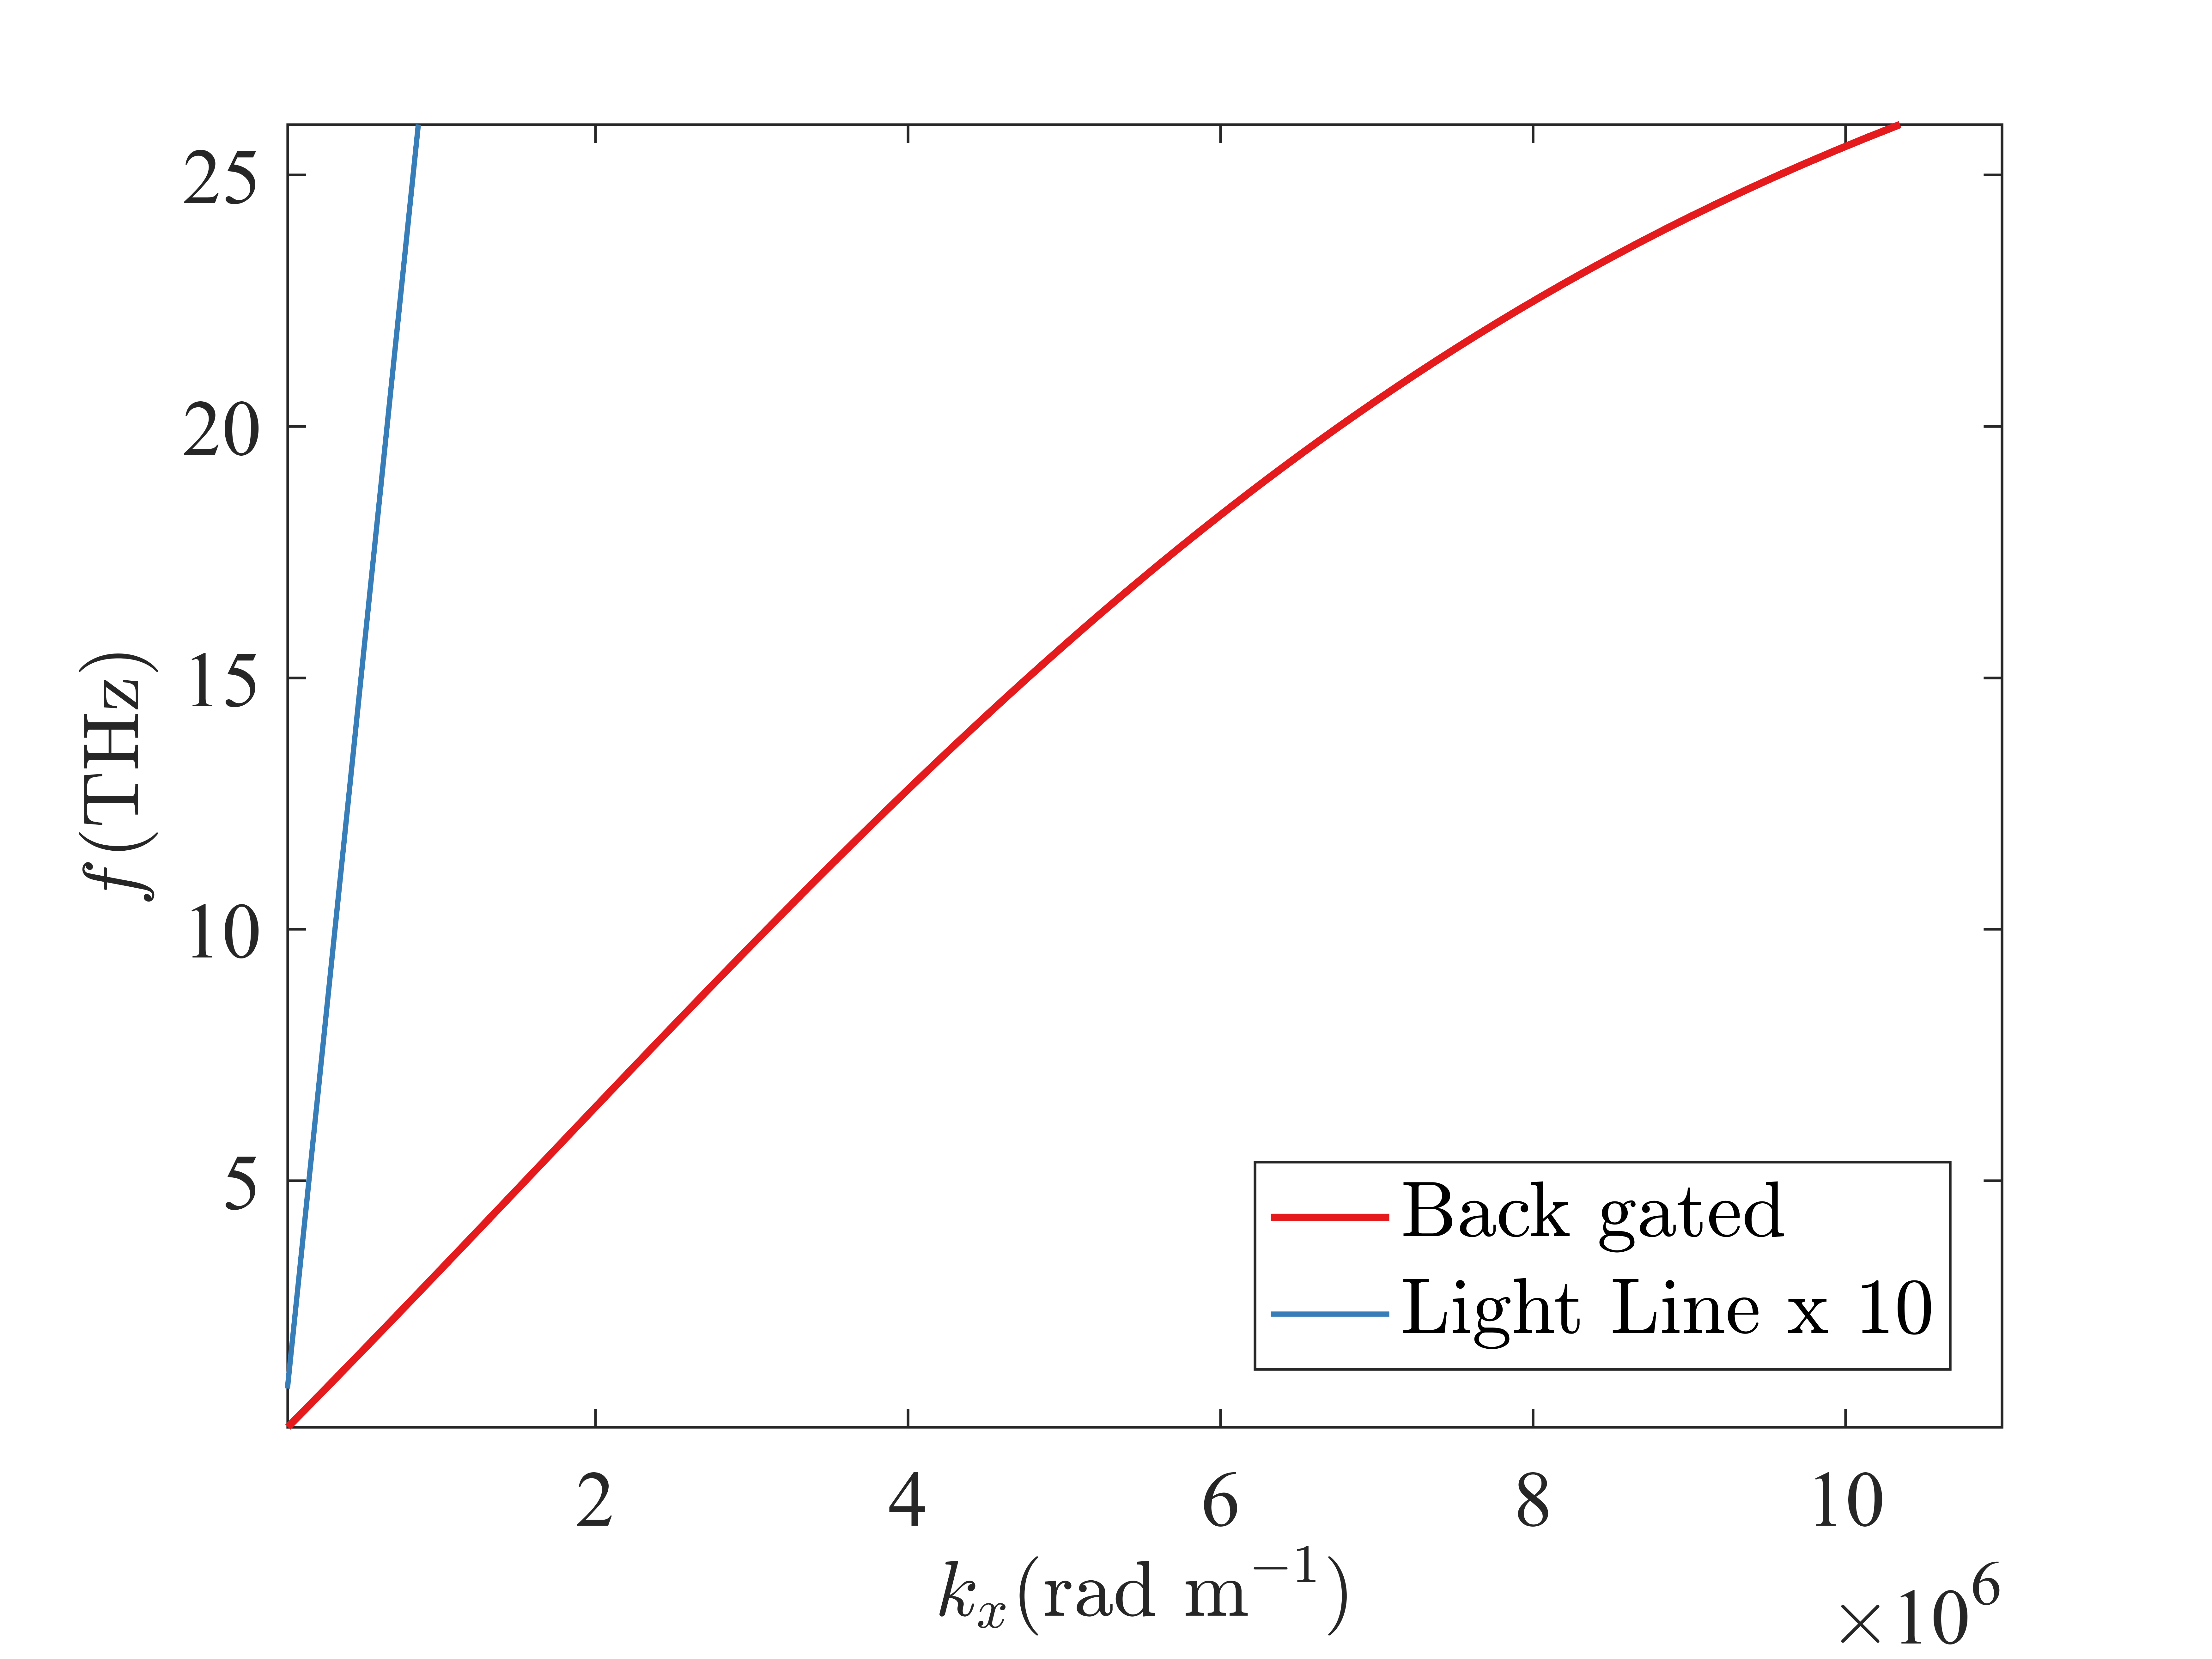
\includegraphics[height=2.2in]{gated_disp.tikz}
      \label{fig:dispersion}}
      \hfil
      \subfloat[]{\includegraphics[height=2.2in]{change_in_freq.tikz}
          \label{fig:tuning}}
  \caption{Dispersion relation of 2DEG embedded in region 2 of the heterostructure. Solid line: real part, dashed line: imaginary part}
  \label{fig:simulation1}
\end{figure}
%
% \begin{figure}
%   \begin{center}
%     \subfloat[]{\def\svgwidth{.45\linewidth}
%     \input{figures/psim_a.pdf_tex}}
%     \label{fig:eps_Ga}
%     \subfloat[Dispersion curve]{\def\svgwidth{.45\linewidth}
%     \input{figures/psim_b.pdf_tex}}
%     \label{fig:eps_Sto}
%   \subfloat[]{\def\svgwidth{.45\linewidth}
%   \input{figures/psim_c.pdf_tex}}
%   \label{fig:eps_Ga}
%   \subfloat[Dispersion curve]{\def\svgwidth{.45\linewidth}
%   \input{figures/psim_d.pdf_tex}}
%   \label{fig:eps_Sto}
%   \\
%   \subfloat[Dispersion curve]{\def\svgwidth{.75\linewidth}
%   \input{figures/psim_result.pdf_tex}}
%   \label{fig:eps_Sto}
%   % \caption{Dielectric Functions of the materials in bulk form. Solid line: real part, dashed line: imaginary part}
%   % \label{fig:eps}
%   \end{center}
% \end{figure}



\end{document}
